\section{Requests}
\label{sec:requests}

The goal of this project is to perform a topology optimisation of a truss structure, minimising the compliance $C$ of the structure subjected to a volume constraint $V - V_0 \le 0$.

The structure is a 2D truss with a fixed geometry and a fixed load as shown in Figure \ref{fig:truss}.

\begin{figure}[H]
    \centering
    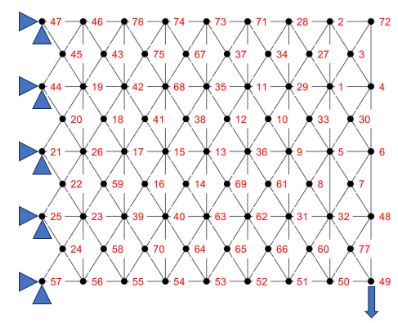
\includegraphics[width=0.7\textwidth]{img/structure.png}
    \caption{Truss structure}
    \label{fig:truss}
\end{figure}

We can summarise the given data as follows:

% \begin{table}
%     \centering
%     \begin{tabular}{|c|c|}
%         \hline
%         \textbf{Parameter} & \textbf{Value} \\
%         \hline
%         $E$ & $1 \times 10^7$ N/m$^2$ \\
%         $A$ & 0.01 m$^2$ \\
%         $V_0$ & 0.1 m$^3$ \\
%         $P$ & 1000 N \\
%         \hline
%     \end{tabular}
%     \caption{Given data}
%     \label{tab:given_data}
% \end{table}


The formal definition of the request is to perform a topology optimisation for the four cases presented in Table \ref{tab:cases}.

\begin{table}[H]
    \centering
    \begin{tabular}{|c|c|c|c|}
        \hline
        \textbf{Case} & \textbf{$\alpha$} & \textbf{Lower bound $[mm^2]$} & \textbf{Upper bound $[mm^2]$} \\
        \hline
        1             & 0.05              & 0.0001                        & 800                           \\
        2             & 0.10              & 0.0001                        & 800                           \\
        3             & 0.15              & 0.0001                        & 800                           \\
        4             & 0.20              & 0.0001                        & 800                           \\
        \hline
    \end{tabular}
    \caption{Optimisation cases}
    \label{tab:cases}
\end{table}

Here, the parameter $\alpha$ is the volume fraction of the structure, defined as $\alpha = \frac{V_0}{V_{max}}$, where $V_{max} = UB \sum_{j=1}^{N_{beams}} l_j$ is the maximum volume of the structure.